\begin{event}{Intermag 2017 - Computational micromagnetics with JOOMMF workshop}{Intermag2017}{Dublin, Ireland, 24 April 2017}{XFEL}{57}{2}{}

\textbf{Main goals.} We introduced the basics of computational micromagnetics as well as taught the participants how to run JOOMMF simulations.

\textbf{\ODK implication.} JOOMMF was developed as a part of the \ODK project and two participants from the \ODK project were present to deliver the workshop (Marijan Beg, and Ryan A. Pepper). The workshop was co-funded by the conference organisers and the EPSRC CCP Computational Magnetism Network (EP/M022668/1) grant. No costs of the workshop were paid from the \ODK funds.

\textbf{Event summary.} In this workshop we provided a brief introduction to computational micromagnetics. We introduced and taught the use of a Python interface to drive the OOMMF simulation package. At the beginning of the workshop, we provided a lecture style introduction, which was followed by practical exercises where attendees had an opportunity to carry out small micromagnetic calculations, modify given examples and ask more specific questions. Several days after the main event, we held a follow up session, where we were able to talk to participants about their specific needs, get requests for features, and get general feedback.

\textbf{Demographic.} We had 57 participants, but the organizers did not allow us to have their personal details.

\textbf{Results and impact.} During the workshop we received the feedback from the participants about our Python interface to OOMMF as well as gained experience which helped us to structure future workshops.

\begin{figure}[ht]
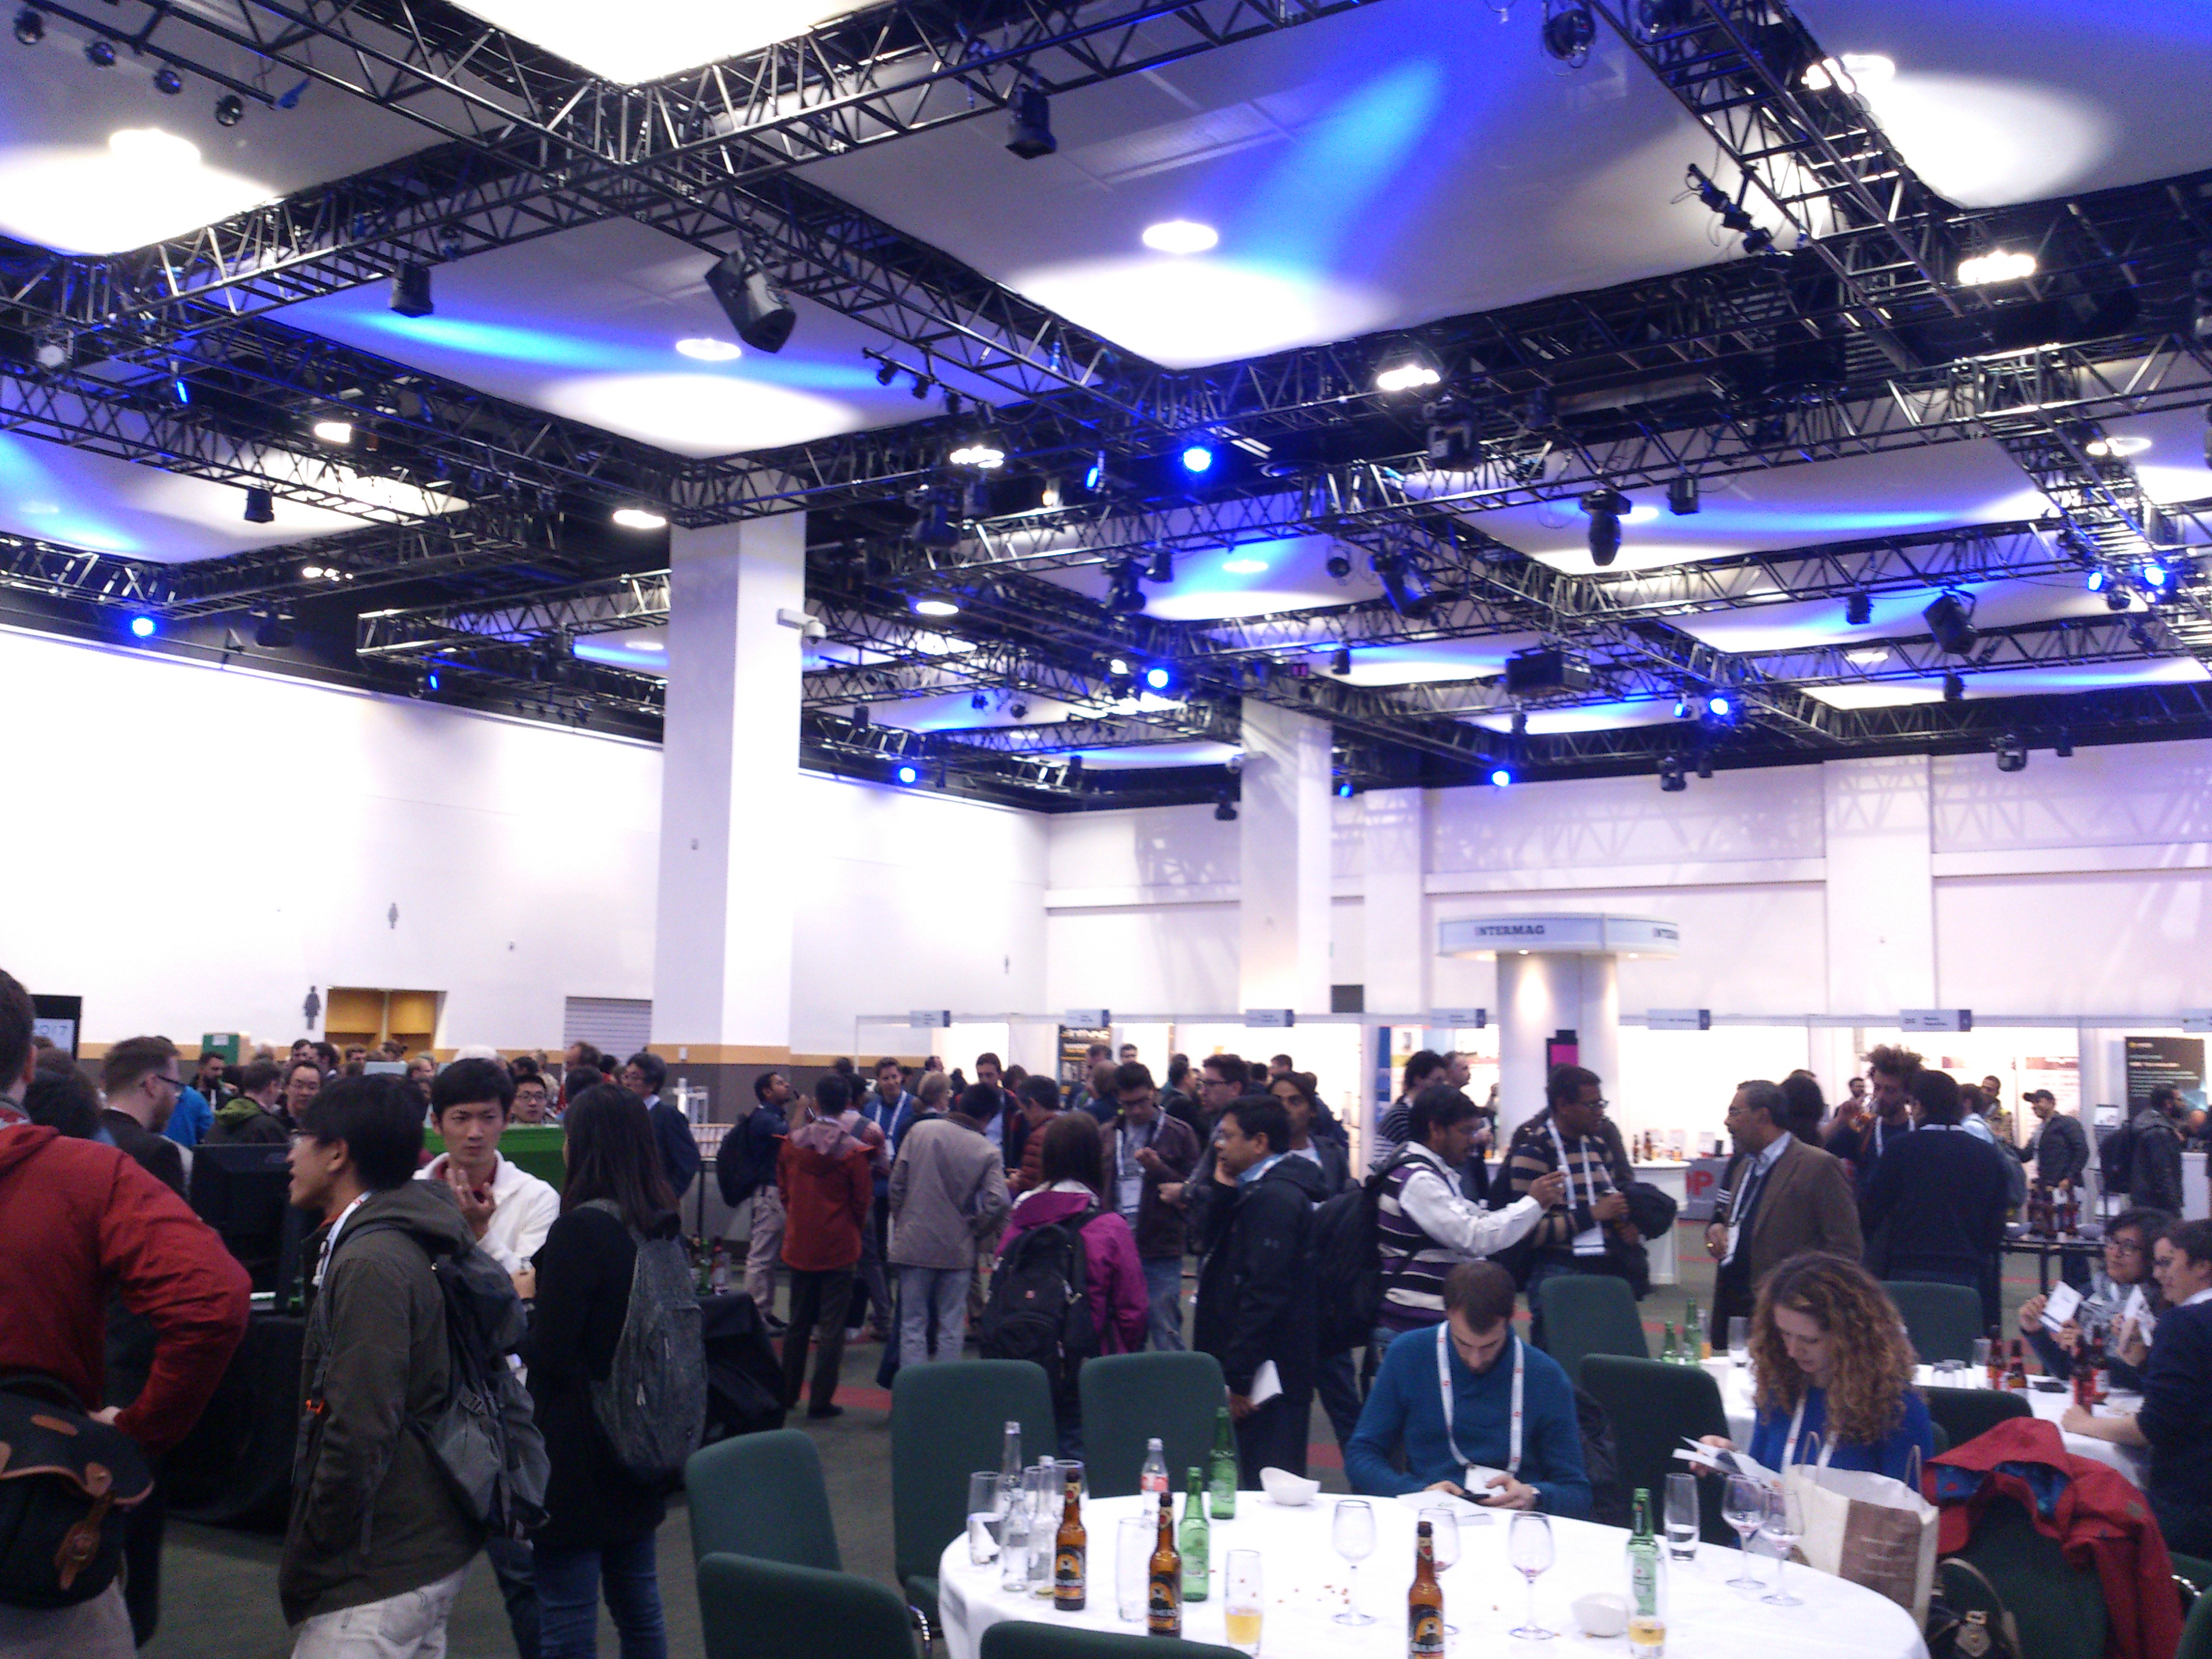
\includegraphics[scale=.1]{IntermagPhoto1.jpg}
\caption*{Intermag2017 conference in Dublin, Ireland.}
\end{figure}

\begin{figure}[ht]
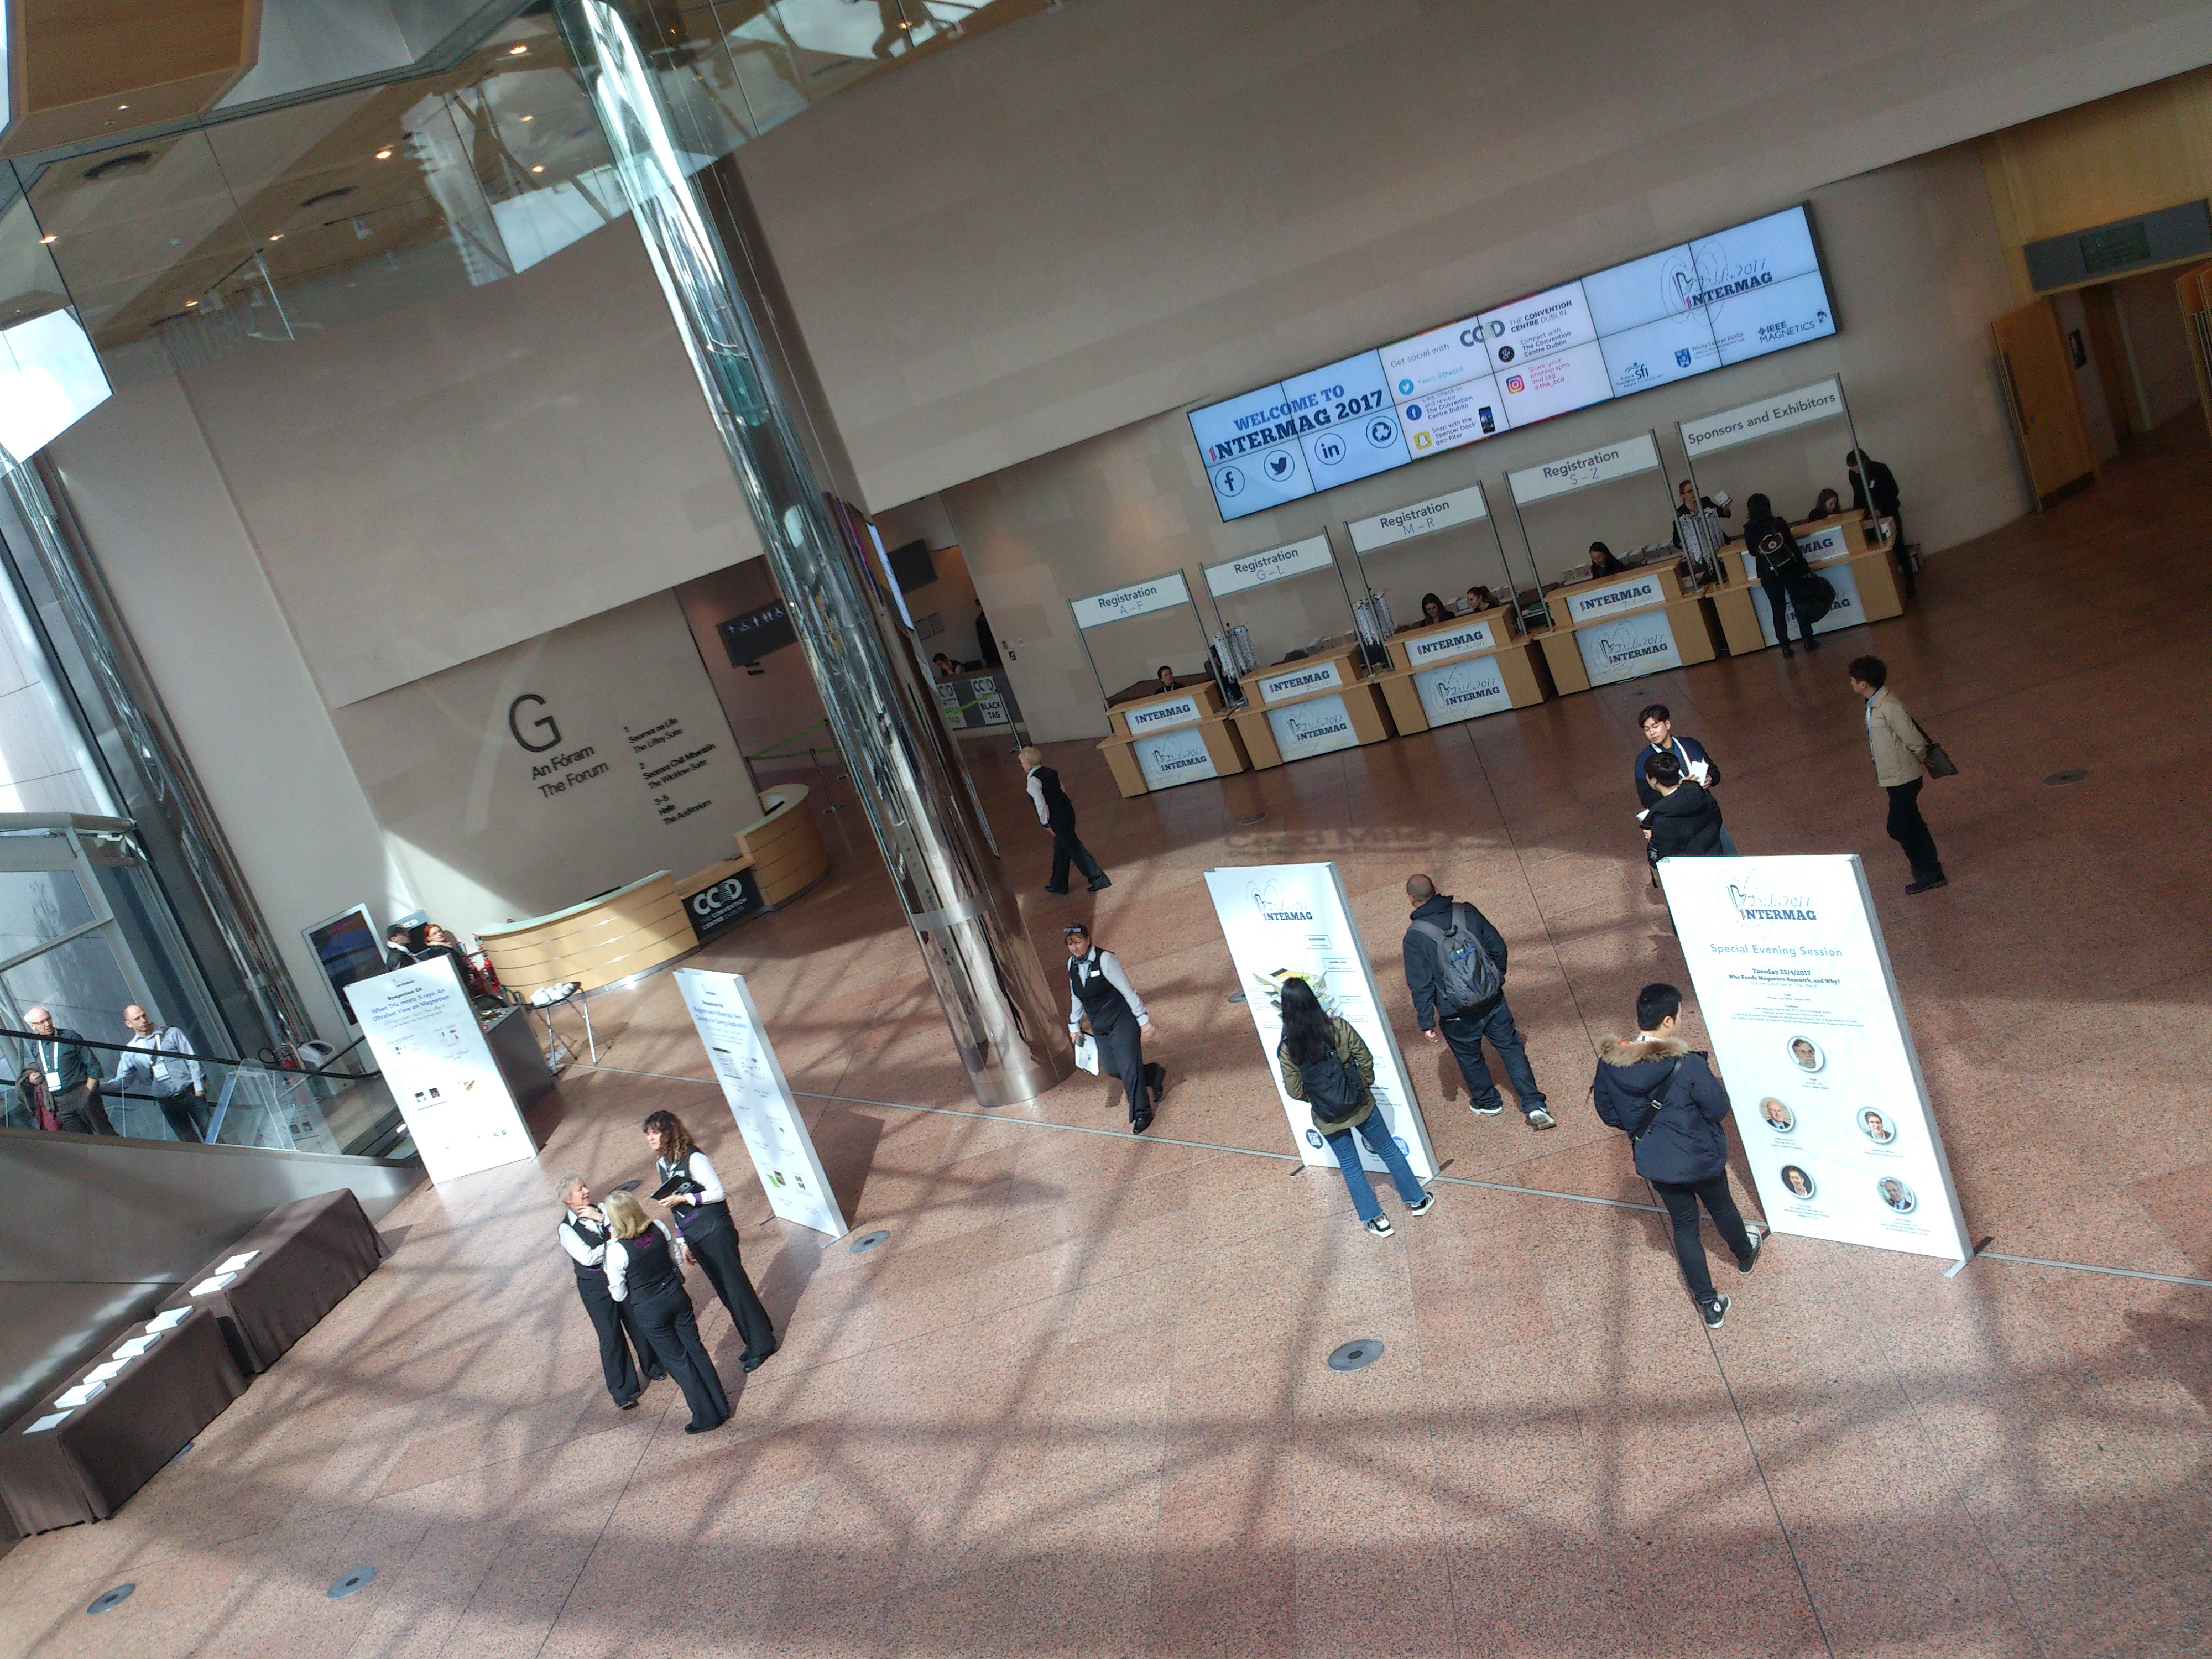
\includegraphics[scale=.1]{IntermagPhoto2.jpg}
\caption*{Intermag2017 conference in Dublin, Ireland.}
\end{figure}

\end{event}
